\documentclass{article}

\usepackage{polski}
\usepackage[margin=1in]{geometry}
\usepackage[parfill]{parskip}
\usepackage{amsmath}
\usepackage{graphicx}
\usepackage{caption}
\usepackage{siunitx}
\usepackage[table,xcdraw]{xcolor}
\usepackage{hyperref}
\usepackage[T1]{fontenc}
\usepackage{comment}
\usepackage{float}
\usepackage{enumerate}

\DeclareSIUnit{\constmag}{\frac{Vs}{Am}}
\DeclareSIUnit{\c}{C^{-1}m^{-1}}

\begin{document}

\begin{center}
\bgroup
\def\arraystretch{1.5}
\begin{tabular}{|c|c|c|c|c|c|}
	\hline
	EAIiIB & \multicolumn{2}{|c|}{\begin{tabular}{@{}c@{}}Stanisław Borowy \\ Maciej Bobrek \end{tabular}} & Rok II & Grupa 1 & Zespół 5 \\
	\hline
	\multicolumn{3}{|c|}{\begin{tabular}{c}Temat: \\ \end{tabular}} & 
	\multicolumn{3}{|c|}{\begin{tabular}{c}Numer ćwiczenia: \\ \end{tabular}} \\
	\hline
	\begin{tabular}{@{}c@{}}Data wykonania \\ 01.01.2023 \end{tabular} & \begin{tabular}{@{}c@{}}Data oddania \\ 02.01.2023 \end{tabular} & 
	\begin{tabular}{c}Zwrot do popr.\\\phantom{data} \end{tabular} & \begin{tabular}{c}Data oddania\\\phantom{data}\end{tabular} &
	\begin{tabular}{c}Data zaliczenia\\\phantom{data}\end{tabular} & \begin{tabular}{c}Ocena\\\phantom{ocena}\end{tabular} \\[4ex]
	\hline
\end{tabular}
\egroup
\end{center}

\section{Cel ćwiczenia}
Cechowanie halotronu przy użyciu pola magnetycznego o znanej indukcji.
Wykorzystanie halotronu do pomiaru przestrzennego rozkładu pola cewki kołowej i magnesu ferrytowego.

\section{Wstęp teoretyczny}

\emph{Napięciem Halla} nazywamy różnicę potencjałów pomiędzy bokami
przewodnika, powstającą w prostopadłym do kierunku przepływu prądu
polu magnetycznym, którego wartość możemy określić za pomocą wzoru
\begin{align}
    U_H = cIB
\end{align}
gdzie $c$ jest stałą halotronu, $I$ natężeniem prądu,
a $B$ indukcją pola magnetycznego.
Dodatkowo definiujemy \emph{halotron} jako urządzenie
wykorzystujące zjawisko napięcia Halla.

Ze względu na budowę halotronu, przy pomiarach napięcia $U$ na jego 
bokach
należy uwzględnić dodatkowe napięcie $U_R$ proporcjonalne do
przepływającego przez niego prądu.
\begin{align}
    U = U_H + U_R = cIB + RI
    \label{eq:Ugen}
\end{align}
$U_R$ można zmierzyć jako wartość napięcia na bokach halotronu, kiedy
nie przepływa przez niego prąd.

Jeżeli źródłem pola magnetycznego jest cewka kołowa o $N$ zwojach, to
wartość indukcji tego pola w danym punkcie przestrzeni możemy
policzyć rozpatrując kilka przypadków.
\begin{enumerate}[I.]
    \item \emph{Środek cewki} -- w tym jednym punkcie wartość indukcji
    pola wynosi
    \begin{align}
        B_0 = \frac{\mu_0NI_S}{2R},
        \label{eq:Bsimple}
    \end{align}
    gdzie $\mu_0$ jest stałą magnetyczną równą $4 \pi \cdot 10^{-7}$ \SI{}{\constmag}, $I_s$ natężeniem płynącym przez zwoje, a $R$
    promieniem zwojów.
    \item \emph{Oś symetrii cewki} -- wtedy indukcja jest funkcją
    odległości $z$ od środka cewki i wynosi
    \begin{align}
    \label{IndukcjaB}
        B(z) = \frac{B_0}{\left(1 + \frac{z^2}{R^2}\right)^{3/2}}.
    \end{align}
    \item \emph{Punkty na średnicy kołowej cewki} -- dzieląc okrąg
    zwoju na $2n$ części możemy zapisać wartość indukcji w odległości
    $y$ od środka cewki jako sumę
    \begin{align}
        B = \frac{\mu_0NI_S}{2Rn}\sum^n_{k=1}\frac{1 - p\cos{\alpha_k}}{(1 - 2p\cos{\alpha_k} + p^2)^{3/2}},
    \end{align}
    gdzie $p = \frac{y}{R}$, a $\alpha_k = \frac{\pi}{n}\left(k - \frac{1}{2}\right)$.
\end{enumerate}
\newpage
Dodatkowo,
\begin{enumerate}[IV.]
    \item indukcję krótkiego magnesu w odległości $z$ od jego środka
    możemy opisać jako
    \begin{align}
        B(z) = \frac{\mu_0\mu}{2\pi z^3},
        \label{eq:Bmag}
    \end{align}
    gdzie $\mu$ jest wartością momentu magnetycznego magnesu.
\end{enumerate}

\section{Aparatura}
Do wykonania ćwiczenia zespół użył 
\begin{enumerate}
    \item Halotron
    \item Zasilacz prądu cewki z regulacją
    \item Potencjometr
    \item Amperomierz
    \item Woltomierz
    \item Miliamperomierz
    \item Zasilacz prądowy halotronu
\end{enumerate}
Podane wyżej komponenty zostały połączone w następujący układ
\begin{figure}[h!]
    \centering
    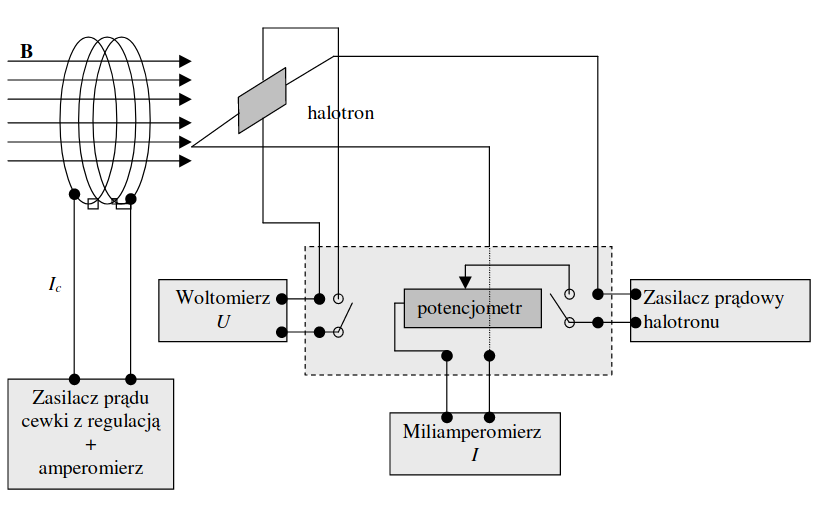
\includegraphics[scale=0.6]{cw43/halotron.png}
    \caption{Schemat wykorzystanego układu pomiarowego}
\end{figure}
\newpage
\section{Wyniki Pomiarów}
Na początku, zespół przesuwał halotron w poziomie, szukając punktu, w którym napięcie na jego bokach będzie maksymalne.
Od tego miejsca analogicznie działano w poziomie, tym razem szukając minimum.
Wynikiem był halotron położony idealnie w centrum cewki o napięciu $U = \SI{4.5}{V}$.

Zespół  wykonał pomiar napięcia U w funkcji natężenia prądu cewki \textit{Is} dla trzech wartości prądu halotronu 
\textit{I}. Wyniki wpisano do tabeli \ref{tab:1}

\begin{table}[!ht]
    \centering
    \renewcommand*{\arraystretch}{1.2}
    \begin{tabular}{|c*{14}{|p{0.8cm}}}
    \hline
        Prąd cewki  \textit{Ic}  [A] & 0 & 1  & 2 & 3 & 4 & 5 & 6 & 7 & 8 & 9 & 10 \\ \hline
        Prąd halotronu \textit{I} [mA] & \multicolumn{11}{|c|}{Napięcie U[mV]} \\ \hline
         7,5 & 0,8 & 1,3 & 1,7 & 2,2 & 2,6 & 3 & 3,4 & 3,9 & 4,3 & 4,8 & 5,3  \\  \hline
        5 & 0,6 & 0,8 & 1,1 & 1,4 & 1,7 & 2 & 2,3 & 2,6 & 2,9 & 3,1 & 3,4  \\  \hline
        3,5 & 0,3 & 0,5 & 0,7 & 0,9 & 1,1 & 1,3 & 1,5 & 1,8 & 2 & 2,2 & 2,4  \\ \hline
    \end{tabular}
    \caption{Tabela Wyników Pomiaru Napięcia}
    \label{tab:1}
\end{table}

Następnie zespół ustalił prąd halotronu \textit{I} i cewki $I_c$ i zaczynając od środka cewki przesuwał halotron co 0,5 cm i odczytywał napięcie U.
Wyniki wpisano  do tabeli  \ref{tab:2} . W tabeli została wpisana policzona Indukcja B ze wzoru \ref{IndukcjaB}
\begin{align*}
    \textit{I}=7,5\si{mA}
\end{align*}
\begin{align*}
    \textit{Ic}=10  \si{A} 
\end{align*}
\begin{table}[H]
    \centering
    \begin{tabular}{|c|c|c|c|c|c|}
    \hline
        Odległość x [cm] & 0 & 0,5 & 1 & 1,5 & 2   \\ \hline
        Napięcie U [mV] & 5,3 & 5,2 & 5,1 & 4,9 & 4,6   \\ \hline
        Indukcja B [T] & 0,003968328 & 0,003968328 & 0,003968328 & 0,003968327 & 0,003968327   \\\hline  \\\hline
        Odległość x [cm] &  2,5 & 3 & 3,5 & 4 & 4,5   \\ \hline
        Napięcie U [mV] & 4,3 & 3,9 & 3,6 & 3,3 &3  \\ \hline
        Indukcja B[T]  & 0,003968327 & 0,003968327 & 0,003968327 & 0,003968327 & 0,003968326  \\\hline  \\\hline
        Odległość x [cm] & 5  & 5,5 & 6,5 & 7 & 7,5     \\\hline
        Napięcie U [mV]  & 2,7& 2,5 & 2,3 & 2,1 & 1,9 \\ \hline
        Indukcja B[T] & 0,003968326 & 0,003968326 & 0,003968325 & 0,003968325 & 0,003968324 \\\hline  \\\hline
        Odległość x [cm]  & 8 & 8,5 & 9 & 9,5 & 10     \\\hline
        Napięcie U [mV]  & 1,8 & 1,7 & 1,6 &1,5 & 1,4  \\ \hline
        Indukcja B[T] & 0,003968324 & 0,003968323 & 0,003968323 & 0,003968322 & 0,003968322 \\ \hline
    \end{tabular}
    \caption{Tabela Wynikiów pomiaru Napięcia i Indukcji}
    \label{tab:2}
\end{table}

Następnie zespół powtórzył pomiary indukcji  pola magnetycznego dla magnesu stałego(ferrytowego) i wyniki wpisal to tabeli \ref{tab:4}
\begin{table}[!ht]
    \centering
    \begin{tabular}{|l|l|l|l|l|l|l|l|l|l|l|l|}
    \hline
        Odległość x [cm] & 0 & 0,5 & 1 & 1,5 & 2 & 2,5 & 3 & 3,5 & 4 & 4,5 & 5 \\ \hline
        Napięcie U [mV] & 179 & 58,6 & 31 & 17,7 & 10,7 & 7,2 & 5 & 3,8 & 3 & 2,4 & 2 \\ \hline
         Indukcja B & ~ & 31,002 & 3,875 & 1,148 & 0,484 & 0,248 & 0,144 & 0,090 & 0,061 & 0,043 & 0,031 \\ \hline
    \end{tabular} 
    \caption{Wyniki Pomiarów dla magnesu ferrytowego}
    \label{tab:4}
\end{table}
\section{Opracowanie wyników pomiarów}

Obliczenia zaczynamy od naniesienia wyników pomiarów z tabeli
\ref{tab:1} na wykres napięcia halotronu $U$ od prądu cewki $I_c$.
Przez zaznaczone punkty prowadzimy prostą, której współczynniki
zostały wyliczone metodą regresji liniowej i wynoszą odpowiednio
\begin{itemize}
    \item Dla prądu halotronu $I = \SI{7.5}{mA}$: $a = 0.441, b = 0.823$
    \item Dla $I = \SI{5}{mA}$: $a = 0.287, b = 0.555$
    \item Dla $I = \SI{3.5}{mA}$: $a = 0.213, b = 0.273$
\end{itemize}
\begin{figure}[h]
    \centering
    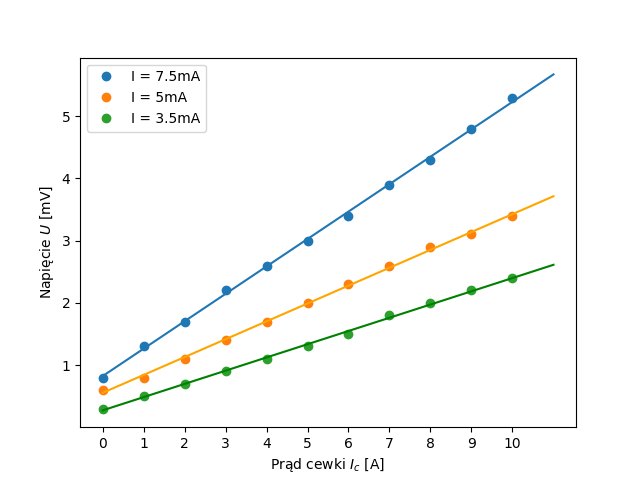
\includegraphics[scale=0.75]{cw43/wykres1.png}
    \caption{Wykres zależności zmierzonego na halotronie napięcia, a
    natężeniem prądu cewki dla różnych wartości natężenia prądu halotronu.}
    \label{fig:fig1}
\end{figure}

Jak wyliczone proste mają się do parametrów halotronu wyznaczymy
łącząc wzór \eqref{eq:Ugen} z \eqref{eq:Bsimple}
\begin{align}
    U(I_c) = \frac{cI\mu_0N}{2R}I_c + RI.
\end{align}
Z tak sformułowanego równania wynika, że 
\begin{align*}
    b &= RI \\
    a &= \frac{cI\mu_0 N}{2R}.
\end{align*}
Oznacza to, że dla każdego wyznaczonego $b$ możemy obliczyć $R$ jako
$R = \frac{b}{I}$, a później, tak obliczone $R$, podstawić do wzoru
z $a$ i obliczyć $c$. Obliczenia przeprowadzamy dla każdego prądu halotronu $I$.
\begin{itemize}
    \item Dla $I = \SI{7.5}{mA}$: $R = \SI{110}{\Omega}, c = \SI{2.57e8}{\c}$
    \item Dla $I = \SI{5}{mA}$: $R = \SI{111}{\Omega}, c = \SI{2.54e8}{\c}$
    \item Dla $I = \SI{3.5}{mA}$: $R = \SI{78}{\Omega}, c = \SI{1.89e8}{\c}$
\end{itemize}
Z tych trzech wartości $R$ i $c$ liczymy odpowiadające im niepewności
standardowe
\begin{align*}
    \bar{R} &= \frac{1}{n}\sum R_i \approx \SI{100}{\Omega} \\
    u(R) &= \sqrt{\frac{\sum(R_i - \bar{R})^2}{n(n - 1)}} \approx \SI{11}{\Omega} \\
    \bar{c} &\approx \SI{2.33e8}{\c} \\
    u(c) &\approx \SI{0.22e8}{\c}.
\end{align*}

Na podstawie wyników z tabeli \ref{tab:2} możemy pokazać dane na wykresie i porównać je z zależnością teoretyczna $B(x)$
\begin{figure}[H]
    \centering
    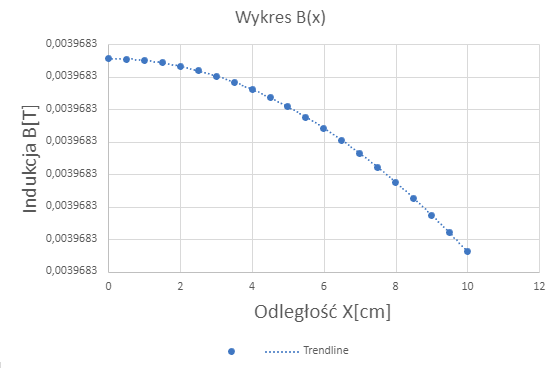
\includegraphics[scale=0.8]{cw43/wykres.png}
    \caption{Wykres zależności Odległości x od Indukcji B}
    \label{fig:fig2}
\end{figure}

Połączenie wzorów \eqref{eq:Ugen} i \eqref{eq:Bmag} daje nam funkcję
napięcia na halotronie $U$ od odległości halotronu od magnesu stałego
$z$.
\begin{align*}
    U = \frac{cI\mu_0\mu}{2\pi} \cdot \frac{1}{z^3} + RI,
\end{align*}
dopasowując zebrane dane w tabeli \ref{} do tej krzywej metodą
regresji liniowej otrzymujemy współczynniki $a = 6.772$ i $b = 7.752$.
Za pomocą tego wyniku możemy wyliczyć $\mu$.
\begin{align*}
    a = \frac{cI\mu_0\mu}{2\pi} \Rightarrow \mu = \frac{2\pi a}{cI\mu_0} = \frac{2 \cdot \pi \cdot 6.772}{2.33 \cdot 10^8 \cdot 4 \cdot \pi \cdot 10^{-7}} \approx \SI{19.376}{Am^2}.
\end{align*}
Tak wyliczone $\mu$ możemy wykorzystać, żeby policzyć indukcję pola
magnetycznego magnesu $B$ dla każdej odległości $z$.

\begin{table}[h]
\centering
\begin{tabular}{|l|l|l|l|l|l|l|l|l|l|l|}
\hline
Odległość z{[}cm{]} & 0,5    & 1     & 1,5   & 2     & 2,5   & 3     & 3,5   & 4     & 4,5   & 5     \\ \hline
Napięcie U{[}mV{]}  & 59,6   & 31    & 17,7  & 10,7  & 7,2   & 5     & 3,8   & 3     & 2,4   & 2     \\ \hline
Indukcja B{[}T{]}   & 31,002 & 3,875 & 1,148 & 0,484 & 0,248 & 0,144 & 0,090 & 0,061 & 0,043 & 0,031 \\ \hline
\end{tabular}
\caption{Obliczenia indukcji pola magnesu $B$ dla każdego pomiaru
odległości $z$ i napięcia halotronu $U$.}
\end{table}
Ponieważ $B$ jest funkcją $z$, aby obliczyć niepewność pomiarową
$u(B)$, potrzebujemy niepewności $u(z)$. Niepewność ta jest wynosi
0.1cm i wynika bezpośrednio z podziałki zastosowanego przyrządu
do mierzenia. Niepewność złożona $u(B)$ wyliczona dla wzoru \eqref{eq:Bmag} wynosi
\begin{align*}
    u(B) = \frac{3\mu_0\mu}{2\pi z^4}u(z) 
    = \frac{3 \cdot 4 \cdot \pi \cdot 10^{-7} \cdot 19.376}{2 \cdot \pi \cdot 2.75^4}10^-3 \approx \SI{0.020}{T}
\end{align*}

\section{Wnioski}
Dzięki wykonanym pomiarom udało nam się ustalić wartości parametrów
znajdującego się w laboratorium halotronu
\begin{itemize}
    \item stała halotronu $c = \SI{2.33e8}{\c} z niepewnością u(c) = \SI{0.22e8}{\c}$
    \item opór cewki $R = \SI{100}{\Omega}$ z niepewnością $u(R) = \SI{11}{\Omega}$.
\end{itemize}
Przeanalizowaliśmy również zależność pomiędzy napięciem pomiędzy
bokami halotronu w zależności od jego odległości od źródła pola
magnetycznego. Zależność ta została zwizualizowana na wykresie
\ref{fig:fig1} i \ref{fig:fig2}.
\end{document}
